\documentclass{beamer}

\usepackage[utf8]{inputenc}

\usepackage{amsmath,amsfonts,amssymb,amsthm}
\usepackage{thmtools}
\usepackage{stmaryrd}
\usepackage{natbib}
\usepackage{url}
\usepackage{array}
\usepackage{arydshln}
\usepackage{ifthen}

\usepackage{todonotes}
\presetkeys{todonotes}{inline}{}

\usepackage{ifpdf}
\usepackage{verbatim}
\usepackage{mathpartir}
\usepackage{listings}
\lstset{
  basicstyle=\ttfamily,
  columns=fullflexible,
  keepspaces=true,
  mathescape
}

\usepackage{rotating}

\usepackage{mathtools}
\DeclarePairedDelimiter\ceil{\lceil}{\rceil}
\DeclarePairedDelimiter\floor{\lfloor}{\rfloor}

\usepackage{appendix}

\usepackage{tikz}
\usepackage{multirow,bigdelim}

%% make latex preview-mode work with natbib...
% \usepackage[displaymath,floats,graphics,textmath,footnotes]{preview}


\newcommand{\forcenewline}{$\phantom{v}$\\}
\newcommand{\judgment}[2]{\paragraph{#1}\hspace{\stretch{1}}\fbox{$#2$}}

\newcommand{\update}[2]{[#1 \mapsto #2]}
\newcommand{\sem}[1]{\left\llbracket #1 \right\rrbracket}

% Math notation
\newcommand{\restrictfun}[1]{|_{#1}}
\newcommand{\parfun}{\rightharpoonup}
\newcommand{\finparfun}{\xrightharpoonup{\textit{\tiny{fin}}}}
\newcommand{\monnefun}{\xrightarrow{\textit{\tiny{mon, ne}}}}
\newcommand{\monfun}{\xrightarrow{\textit{\tiny{mon}}}}
\newcommand{\nefun}{\xrightarrow{\textit{\tiny{ne}}}}
\newcommand{\fun}{\rightarrow}
\newcommand{\defeq}{\stackrel{\textit{\tiny{def}}}{=}}
\newcommand{\nequal}[1][n]{\stackrel{\tiny{#1}}{=}}
\renewcommand{\nsim}[1][n]{\stackrel{\tiny{#1}}{\simeq}}

\newcommand\subsetsim{\mathrel{\ooalign{\raise.2ex\hbox{$\subset$}\cr
      \hidewidth\lower.8ex\hbox{\scalebox{0.9}{$\sim$}}\hidewidth\cr}}}
\newcommand\supsetsim{\mathrel{\ooalign{\raise.2ex\hbox{$\supset$}\cr
      \hidewidth\lower.8ex\hbox{\scalebox{0.9}{$\sim$}}\hidewidth\cr}}}
\newcommand{\nsubsim}[1][n]{\stackrel{\tiny{#1}}{\subsetsim}}
\newcommand{\nsupsim}[1][n]{\stackrel{\tiny{#1}}{\supsetsim}}

\newcommand{\nsubeq}[1][n]{\stackrel{\tiny{#1}}{\subseteq}}
\newcommand{\nsupeq}[1][n]{\stackrel{\tiny{#1}}{\supseteq}}

\newcommand{\union}{\mathbin{\cup}}
\DeclareMathOperator{\dom}{dom}
\newcommand{\blater}{\mathop{\blacktriangleright}}
\newcommand{\id}{\var{id}}
\newcommand{\undefined}{\mathit{undefined}}

\newcommand{\powerset}[1]{\mathcal{P}(#1)}

\newcommand{\false}{\mathit{false}}
\newcommand{\true}{\mathit{true}}


% cofes
\newcommand{\cofe}{c.o.f.e.}
\newcommand{\cofes}{\cofe{}'s}
\newcommand{\CatC}{\mathbb{C}}
\newcommand{\CatP}{\mathbb{P}}

% Comments
\newcommand\lau[1]{{\color{purple} \sf \footnotesize {LS: #1}}\\}
\newcommand\dominique[1]{{\color{purple} \sf \footnotesize {DD: #1}}\\}
\newcommand\lars[1]{{\color{purple} \sf \footnotesize {LB: #1}}\\}

% Variables
\newcommand{\var}[1]{\mathit{#1}}
\newcommand{\hs}{\var{ms}}
\newcommand{\ms}{\hs}
\newcommand{\hv}{\var{hv}}
\newcommand{\rv}{\var{rv}}
\newcommand{\lv}{\var{lv}}
\newcommand{\gl}{\var{g}}
\newcommand{\pc}{\mathit{pc}}
\newcommand{\pcreg}{\mathrm{pc}}
\newcommand{\addr}{\var{a}}
\newcommand{\offset}{\var{offset}}
\newcommand{\word}{\var{w}}
\newcommand{\start}{\var{base}}
\newcommand{\addrend}{\var{end}}
\newcommand{\pwlv}{\var{pwl}}
\newcommand{\mem}{\var{mem}}
\newcommand{\reg}{\var{reg}}
\newcommand{\heapseg}{\var{ms}}
\newcommand{\heap}{\var{mem}}
\newcommand{\perm}{\var{perm}}
\newcommand{\permp}{\var{permPair}}
\newcommand{\roll}{\var{roll}}
\newcommand{\instr}{\var{instr}}
\newcommand{\stdcap}[1][(\perm,\gl)]{\left(#1,\start,\addrend,\addr \right)}
\newcommand{\adv}{\var{adv}}
\newcommand{\msframe}{ms_\var{frame}}
\newcommand{\link}{\var{link}}
\newcommand{\stk}{\var{stk}}
\newcommand{\flag}{\var{flag}}
\newcommand{\nwl}{\var{nwl}}
\newcommand{\pwl}{\var{pwl}}
\newcommand{\sta}{\var{sta}}
\newcommand{\cnst}{\var{cnst}}
\newcommand{\olf}{\var{offsetLinkFlag}}
\newcommand{\prp}{\var{prp}}

% Memory projections
\newcommand{\plainproj}[1]{\mathrm{#1}}
\newcommand{\memheap}[1][\Phi]{#1.\plainproj{mem}}
\newcommand{\memreg}[1][\Phi]{#1.\plainproj{reg}}

\newcommand{\updateHeap}[3][\Phi]{#1\update{\plainproj{mem}.#2}{#3}}
\newcommand{\updateReg}[3][\Phi]{#1\update{\plainproj{reg}.#2}{#3}}

% Configuration end states
\newcommand{\failed}{\textsl{failed}}
\newcommand{\halted}{\textsl{halted}}

% Functions
\newcommand{\plainfun}[2]{
  \ifthenelse{\equal{#2}{}}
  {\mathit{#1}}
  {\mathit{#1}(#2)}
}
\newcommand{\decode}{\plainfun{decode}{}}
\newcommand{\encode}{\plainfun{encode}{}}
\newcommand{\encodePerm}{\mathit{encodePerm}}
\newcommand{\encodePermPair}{\plainfun{encodePermPair}{}}
\newcommand{\encodeLoc}{\mathit{encodeLoc}{}}
\newcommand{\decodePermPair}{\plainfun{decodePermPair}}
\newcommand{\decodePerm}[1]{\plainfun{decodePerm}{#1}}
\newcommand{\updatePcPerm}[1]{\plainfun{updatePcPerm}{#1}}

\newcommand{\executeAllowed}[1]{\plainfun{executeAllowed}{#1}}
\newcommand{\nonZero}[1]{\plainfun{nonZero}{#1}}
\newcommand{\readAllowed}[1]{\plainfun{readAllowed}{#1}}
\newcommand{\writeAllowed}[1]{\plainfun{writeAllowed}{#1}}
\newcommand{\withinBounds}[1]{\plainfun{withinBounds}{#1}}
\newcommand{\stdUpdatePc}[1]{\plainfun{updatePc}{#1}}

\newcommand{\readCond}[1]{\plainfun{readCondition}{#1}}
\newcommand{\writeCond}[1]{\plainfun{writeCondition}{#1}}
\newcommand{\execCond}[1]{\plainfun{executeCondition}{#1}}
\newcommand{\entryCond}[1]{\plainfun{enterCondition}{#1}}

\newcommand{\revokeTemp}[1]{\plainfun{revokeTemp}{#1}}
\newcommand{\erase}[2]{\floor*{#1}_{\{#2\}}}
\newcommand{\activeReg}[1]{\plainfun{active}{#1}}

% World operations
\newcommand{\future}{\mathbin{\sqsupseteq}}
\newcommand{\pub}{\var{pub}}
\newcommand{\priv}{\var{priv}}
\newcommand{\futurewk}{\mathbin{\sqsupseteq}^{\var{pub}}}
\newcommand{\futurestr}{\mathbin{\sqsupseteq}^{\var{priv}}}
\newcommand{\heapSat}[3][\heap]{#1 :_{#2} #3}
\newcommand{\memSat}[3][n]{\heapSat[#2]{#1}{#3}}
\newcommand{\memSatPar}[4][n]{\heapSat[#2]{#1 , #4}{#3}}

\newcommand{\monwknefun}{\xrightarrow[\text{\tiny{$\futurewk$}}]{\textit{\tiny{mon, ne}}}}
\newcommand{\monstrnefun}{\xrightarrow[\text{\tiny{$\futurestr$}}]{\textit{\tiny{mon, ne}}}}


% Assembly labels
\newcommand{\codelabel}[1]{\mathit{#1}}
\newcommand{\init}{\codelabel{init}}
\newcommand{\malloc}{\codelabel{malloc}}
\newcommand{\counter}{\codelabel{counter}}
\newcommand{\iocap}{\codelabel{iocap}}

% Type(s)
\newcommand{\type}[1]{\mathrm{#1}}
\newcommand{\asmType}{\plaindom{AsmType}}


% Domains
\newcommand{\plaindom}[1]{\mathrm{#1}}
\newcommand{\Caps}{\plaindom{Cap}}
\newcommand{\Words}{\plaindom{Word}}
\newcommand{\Addrs}{\plaindom{Addr}}
\newcommand{\ExecConfs}{\plaindom{ExecConf}}
\newcommand{\RegName}{\plaindom{RegisterName}}
\newcommand{\Regs}{\plaindom{Reg}}
\newcommand{\Heaps}{\plaindom{Mem}}
\newcommand{\Mems}{\Heaps}
\newcommand{\HeapSegments}{\plaindom{MemSegment}}
\newcommand{\MemSegments}{\HeapSegments}
\newcommand{\Confs}{\plaindom{Conf}}
\newcommand{\Instrs}{\plaindom{Instructions}}
\newcommand{\nats}{\mathbb{N}}
\newcommand{\ints}{\mathbb{Z}}
\newcommand{\Perms}{\plaindom{Perm}}
\newcommand{\Globals}{\plaindom{Global}}

\newcommand{\Rel}{\plaindom{Rel}}
\newcommand{\Rels}{\plaindom{Rels}}
\newcommand{\States}{\plaindom{State}}
\newcommand{\RegionNames}{\plaindom{RegionName}}
\newcommand{\Regions}{\plaindom{Region}}
\newcommand{\Reg}{\plaindom{Reg}}
\newcommand{\Worlds}{\plaindom{World}}
\newcommand{\Wor}{\plaindom{Wor}}
\newcommand{\Worwk}{\Wor_{\futurewk}}
\newcommand{\Worstr}{\Wor_{\futurestr}}
\newcommand{\xiwk}{\xi_{\var{wk}}}
\newcommand{\xistr}{\xi_{\var{str}}}
\newcommand{\StorePred}{\plaindom{MemSegPred}}
\newcommand{\UPred}[1]{\plaindom{UPred}(#1)}
\newcommand{\DCPred}[1]{\plaindom{P}^\downarrow(#1)}

\newcommand{\Views}{\plaindom{View}}

% LR
\newcommand{\intr}[2]{\mathcal{#1}}
\newcommand{\valueintr}[1]{\intr{V}{#1}}
\newcommand{\exprintr}[1]{\intr{E}{#1}}
\newcommand{\contintr}[1]{\intr{K}{#1}}
\newcommand{\regintr}[1]{\intr{R}{#1}}
\newcommand{\stdvr}{\valueintr{\asmType}}
\newcommand{\stder}{\exprintr{\asmType}}
\newcommand{\stdrr}{\regintr{\asmType}}
\newcommand{\stdkr}{\contintr{\asmType}}
\newcommand{\observations}{\mathcal{O}}
\newcommand{\npair}[2][n]{\left(#1,#2 \right)}

% Reference register/memory
\newcommand{\refreg}[1]{#1}
\newcommand{\refheap}[1]{#1}

% Instructions
% No arguments
\newcommand{\zinstr}[1]{\mathtt{#1}}
\newcommand{\fail}{\zinstr{fail}}
\newcommand{\halt}{\zinstr{halt}}
% One argument
\newcommand{\oneinstr}[2]{\zinstr{#1} \; #2}
\newcommand{\jmp}[1]{\oneinstr{jmp}{#1}}
% Two arguments
\newcommand{\twoinstr}[3]{\zinstr{#1} \; #2 \; #3}
\newcommand{\restricttwo}[2]{\twoinstr{restrict}{#1}{#2}}
\newcommand{\jnz}[2]{\twoinstr{jnz}{#1}{#2}}
\newcommand{\isptr}[2]{\twoinstr{isptr}{#1}{#2}}
\newcommand{\geta}[2]{\twoinstr{geta}{#1}{#2}}
\newcommand{\getb}[2]{\twoinstr{getb}{#1}{#2}}
\newcommand{\gete}[2]{\twoinstr{gete}{#1}{#2}}
\newcommand{\getp}[2]{\twoinstr{getp}{#1}{#2}}
\newcommand{\getl}[2]{\twoinstr{getl}{#1}{#2}}
\newcommand{\move}[2]{\twoinstr{move}{#1}{#2}}
\newcommand{\store}[2]{\twoinstr{store}{#1}{#2}}
\newcommand{\load}[2]{\twoinstr{load}{#1}{#2}}
\newcommand{\lea}[2]{\twoinstr{lea}{#1}{#2}}
% Three arguments
\newcommand{\threeinstr}[4]{\zinstr{#1} \; #2 \; #3 \; #4}
\newcommand{\restrict}[3]{\threeinstr{restrict}{#1}{#2}{#3}}
\newcommand{\subseg}[3]{\threeinstr{subseg}{#1}{#2}{#3}}
\newcommand{\plus}[3]{\threeinstr{plus}{#1}{#2}{#3}}

% Permissions
\newcommand{\plainperm}[1]{\mathrm{#1}}
\newcommand{\noperm}{\plainperm{o}}
\newcommand{\readonly}{\plainperm{ro}}
\newcommand{\readwrite}{\plainperm{rw}}
\newcommand{\exec}{\plainperm{rx}}
\newcommand{\entry}{\plainperm{e}}
\newcommand{\rwx}{\plainperm{rwx}}
% PWL permissions
\newcommand{\readwritel}{\plainperm{rwl}}
\newcommand{\rwl}{\readwritel}
\newcommand{\rwlx}{\plainperm{rwlx}}
\newcommand{\writeloc}{\plainperm{wl}}

% Global/local
\newcommand{\local}{\plainperm{local}}
\newcommand{\glob}{\plainperm{global}}

\newcommand{\localityReg}{\var{localityReg}}
\newcommand{\localReg}{\var{localReg}}
\newcommand{\globalReg}{\var{globalReg}}

% Views
\newcommand{\plainview}[1]{\mathrm{#1}}
\newcommand{\perma}{\plainview{perm}}
\newcommand{\temp}{\plainview{temp}}
\newcommand{\revoked}{\plainview{revoked}}

% OP sem
\newcommand{\diverge}[1][n]{\not\Downarrow_{#1}}
\newcommand{\step}[1][]{\rightarrow_{#1}}

% Conv defs
\newcommand{\lookingat}[3]{\ensuremath{#1} \text{ is looking at } \ensuremath{#2} \text{ followed by } \ensuremath{#3}}
\newcommand{\pointstostack}[3]{\ensuremath{#1} \text{ points to stack with } \ensuremath{#2} \text{ used and } \ensuremath{#3} \text{ unused}}

% Macros
\newcommand{\scall}[3]{\mathtt{scall} \; #1(#2,#3)}


\lstset{basicstyle=\footnotesize\ttfamily,breaklines=true}

\AtBeginSection[]
{
  \begin{frame}<beamer>
    \frametitle{Road map}
    \tableofcontents[currentsection]
  \end{frame}
}

\newsavebox{\locstatebox}
\newsavebox{\tdbox}
\newsavebox{\continuationbox}
\newsavebox{\awkwardex}

\title{Enforcing Well-Bracketed Control Flow on a Capability Machine using Local Capabilities}
\author{Lau Skorstengaard\inst{1} \and Dominique Devriese\inst{2} \and Lars Birkedal\inst{1}}
\institute{\inst{1}Aarhus University \and \inst{2}imec-DistriNet, KU Leuven}
\date{SCM, January 15, 2017}


\begin{document}
\begin{frame}
  \titlepage
\end{frame}

\begin{frame}
  \frametitle{Why capability machines?}
  \begin{itemize}
  \item Interesting compilation target
    \begin{itemize}
    \item C-like calling convention
    \item Enforcement of well-bracketed calls
    \end{itemize}
    
  \item Subject of systems research
    \begin{itemize}
    \item CHERI
    % How do we formally reason about it
    % - One can program anything?
    \end{itemize}
  \end{itemize}
  % The Gap (Derek talk)
\end{frame}

\begin{frame}
  \frametitle{Talk outline}
  \tableofcontents
\end{frame}

\section{A simple capability machine}
% Gradually introduce system
\begin{frame}
  \frametitle{Memory capabilities}
  Challenge:
  \begin{itemize}
  \item Low-level machines provide no means to enforce fine-grained access control.
    % To some extend, you can try to access any memory location you please. (whether or not you are supposed to)
  \end{itemize}
  \pause
  Solution:
  \begin{itemize}[<+->]
  \item Assembly language that uses capabilities instead of pointers
  \item Tagged memory
  \item Capabilities $(\perm,\start,\addrend,\addr)$
    \begin{itemize}
    \item<3-> Permission e.g.\ read ($r$), write ($w$), execute ($x$)
    \item<3-> Range of authority
    \item<3-> Pointer
    \end{itemize}
    % Capabilities are tagged and the tag is tracked throughout execution
  \item Capability aware instructions enforce capability permissions
  \end{itemize}
  \begin{mathpar}
    \inferrule{
      \only<6->{\var{w} = \memreg(r_2)}
      \only<5>{\phantom{\var{w} = \memreg(r_2)}} \\
      % 
      \only<7->{\memreg(r_1) = (\perm,\start,\addrend,\addr)}
      \only<5-6>{\phantom{\memreg(r_1) = (\perm,\start,\addrend,\addr)}}\\
      % 
      \only<8->{\perm \in \{\readwrite, \rwx \}} 
      \only<5-7>{\phantom{\perm \in \{\readwrite, \rwx \} }} \\
      % 
      \only<9->{\start \leq \addr \leq \addrend} 
      \only<5-8>{\phantom{\start \leq \addr \leq \addrend}}
    }
    {\sem{\store{\refreg{r_1}}{\refheap{r_2}}}(\Phi) = 
      \only<6->{\updateHeap{\only<2>{?}\only<3->{\addr}}{\var{w}}}
      \only<5>{\phantom{\updateHeap{\only<2>{?}\only<3->{\addr}}{\var{w}}}}
    }
  \end{mathpar}
\end{frame}

\begin{frame}
  \frametitle{Enter capabilities}
  Challenge:
  \begin{itemize}
  \item Execute capabilities provide no encapsulation: how can we give the
    callee more authority than caller?
  \end{itemize}
  % No way to control how execute capabilities are used
  % - Needed for distrusting parties to set up interface.
  % - One might try to start execution from an arbitrary address.
  % From the M-machine
  Solution (from M-Machine):
  \begin{itemize}
  \item Enter capability:
    \begin{itemize}
    \item Completely opaque, you can only jump to it
    \item Becomes rx when jumped to
      % Cannot read from it, write to it, or manipulate it to point to a new address.
    \end{itemize}
  \item $\sim$ encapsulated closure
  \item Security boundaries
    % Enter capabilities can be seen as a way to set up and cross security boundaries. 
    % When one jumps to an enter capability, then control is lost.
  \item Modularisation
    % Execution must start at the address pointed to.
    % - We only need to make sure that execution does the right thing starting from one address rather than all in the range of authority.
  \end{itemize}
\end{frame}

\begin{frame}
  \frametitle{Local capabilities}
  Challenge:
  \begin{itemize}
  \item Capabilities are irrevocable. 
  \end{itemize}
  % Capabilities are irrevocable.
  % - when a capability is passed to an adversary, then we have to assume that they keep it indefinitly
  % If we want to ensure well-bracketedness, we cannot allow an adversary to capture return capabilities.
  % From CHERI
  Solution (from CHERI):
  \begin{itemize}
  \item Local capabilities (form of temporal information-flow control)
  \item Capabilities extended with a \emph{local} tag and a \emph{permit write local} permission ($\writeloc$)
    % We call a non-local capability global
  \item Local capabilities can only be written to memory through a $\writeloc$ capability
  \item (to make it useful:) $\writeloc$-capabilities must be local themselves
  \end{itemize}
  \begin{mathpar}
    \inferrule{
      \var{w} = \memreg(r_2)\\
      % 
      \memreg(r_1) = \stdcap\\
      % 
      \perm \in \{\readwrite, \rwx, \only<1>{\phantom{\rwl, \rwlx}} \only<2->{\rwl, \rwlx} \}\\
      % 
      \start \leq \addr \leq \addrend\\
      % 
      \only<3->{w=((\_,\local),\_,\_,\_) \only<4->{\Rightarrow \perm \in \{\rwl,\rwlx \}} }
      \only<1-3>{\phantom{\only<1-2>{w=((\_,\local),\_,\_,\_) }\Rightarrow \perm \in \{\rwl,\rwlx \}} }
    }
    {\sem{\store{\refreg{r_1}}{\refheap{r_2}}}(\Phi) = 
      \updateHeap{\addr}{\var{w}}
    }
  \end{mathpar}
\end{frame}

\section{Applications}
\subsection{Enforcing well-bracketedness}
\begin{frame}
  \frametitle{Enforcing well-bracketedness (without a trusted stack)}
  Basic Idea:
  \begin{itemize}
  \item Stack pointer as local $\rwlx$-capability
      % Important that there are NO global rwlx capabilities
      % would undermine the temporal revocation provided by local capabilities.
    \begin{itemize} 
    \item Only place one can store local capabilities
      % Used to store local state
      % (Used in calling convention to store "private" registers content, return address in program, stack capability, and  initial restoration code)
    \end{itemize}
  \item Return pointer as local $\entry$-capability
  \end{itemize}

  Many details to get right:
  \begin{itemize}
  \item Clear non-argument registers upon invocations
      % Makes sure that local capabilities are not passed between calls
  \item Clear part of the stack the callee gains control over
  \item Adversary callbacks must be global
  \end{itemize}
  
  Results:
  \begin{itemize}
  \item Provably enforce well-bracketed control flow and local state
    encapsulation, without a trusted stack!
  \item (Even with a trusted stack, some points above still needed.)
  \end{itemize}
\end{frame}

\begin{comment}
\subsection{Other Examples}
% I already have well-bracketedness.
% The question is whether I want the ticket dispenser and compartmentalisation
\begin{frame}
  \frametitle{More Examples}
  \begin{itemize}
  \item Ticket dispenser
    \begin{itemize}
    \item Compartmentalisation
    \item Local state encapsulated
    \item enter capability
    \end{itemize}
  \item ``Awkward'' %Well-bracketedness, not awkward, only mention, why is well-bracketedness difficult
    \begin{itemize}
    \item Well-bracketedness
    \item Stack as local capability
      \begin{itemize}
      \item Execute code on stack
      \end{itemize}
    \item Return pointer as local
    \item Global call-back
    \end{itemize}
  \end{itemize}
\end{frame}
\end{comment}


\section{Logical Relation}
\subsection{Kripke Worlds}
\begin{frame}
  % Add a figure illustrating this or replace this with a figure
  \frametitle{Kripke Worlds}
  \begin{overprint}
    \onslide<1>
    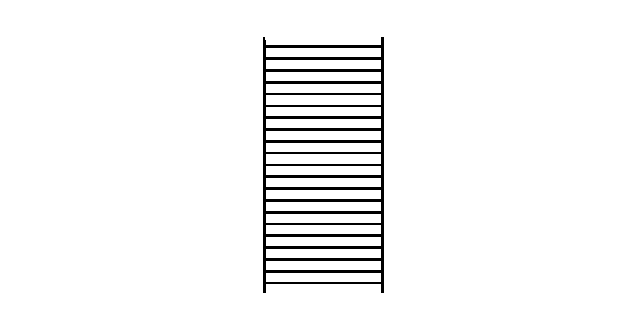
\includegraphics{Worlds/w1.eps}
    \onslide<2>
    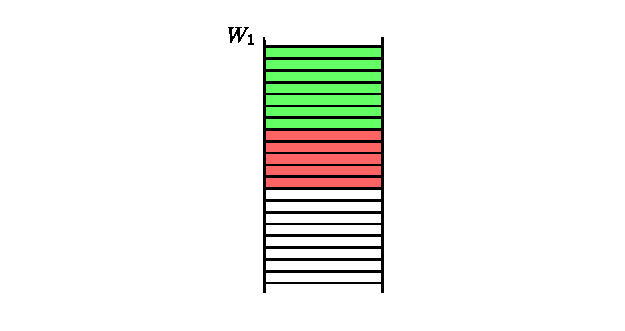
\includegraphics{Worlds/w2.eps}
    \onslide<3>
    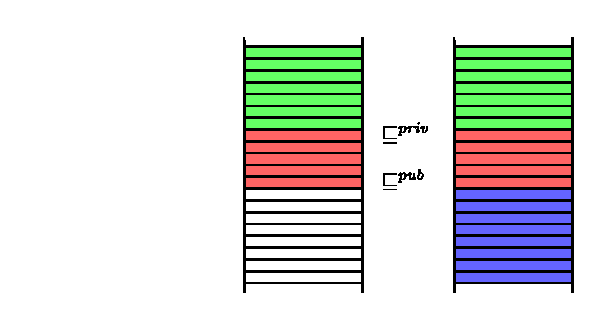
\includegraphics{Worlds/w3.eps}
    \onslide<4>
    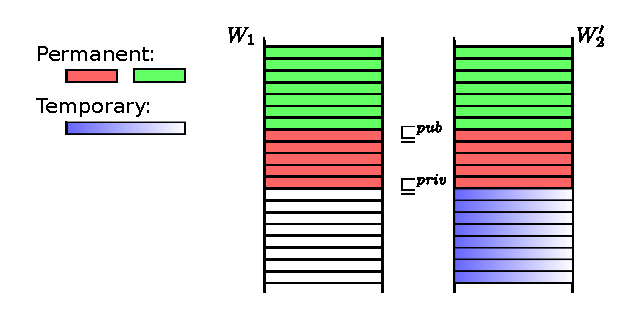
\includegraphics{Worlds/w4.eps}
    \onslide<5>
    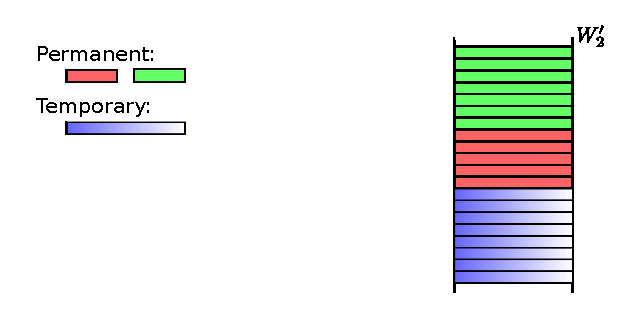
\includegraphics{Worlds/w5.eps}
    \onslide<6>
    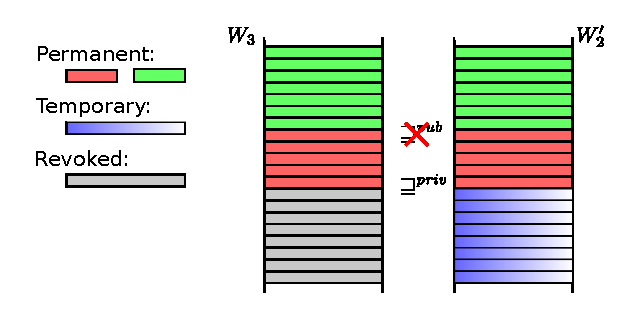
\includegraphics{Worlds/w6.eps}
    \onslide<7>
    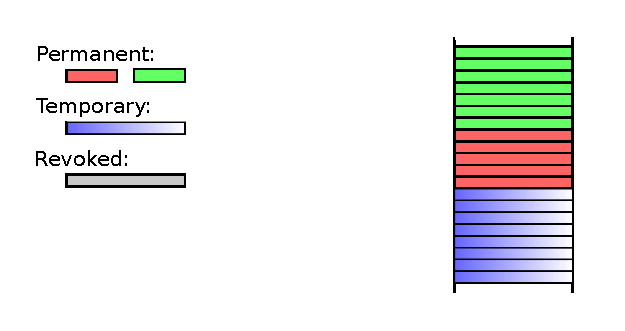
\includegraphics{Worlds/w7.eps}
    \onslide<8>
    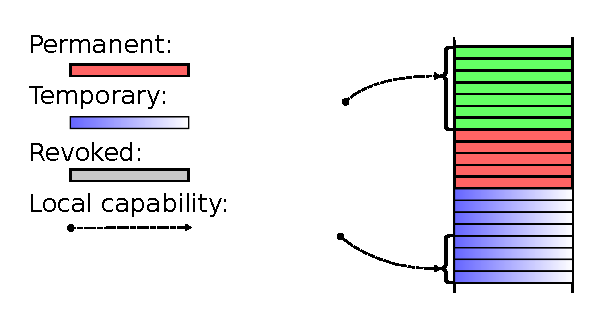
\includegraphics{Worlds/w8.eps}
    \onslide<9>
    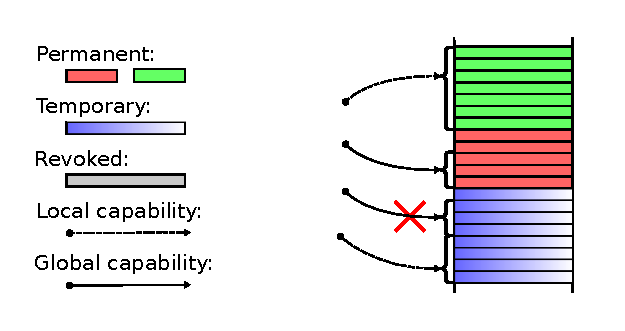
\includegraphics{Worlds/w9.eps}
    \onslide<10>
    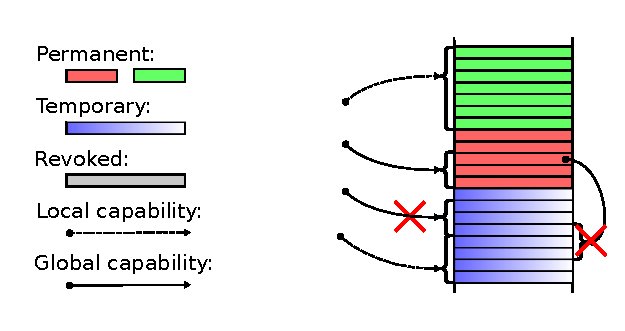
\includegraphics{Worlds/w10.eps}
    \onslide<11>
    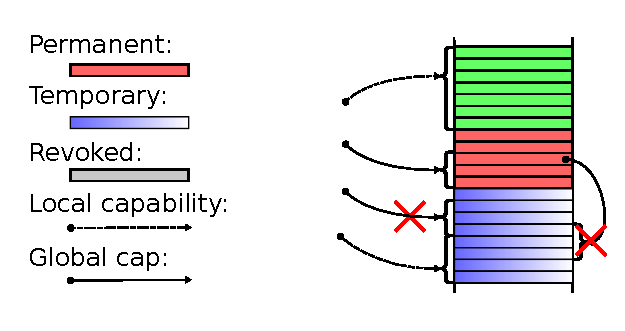
\includegraphics{Worlds/w11.eps}

  \end{overprint}
    \begin{itemize}
    \item Recursive Kripke world
    \item Regions model evolvable invariants (protocols) on memory
      \begin{itemize}
      \item State machines with public and private transitions
      \end{itemize}
    \item Regions are \emph{permanent} or \emph{temporary}
      \begin{itemize}
      \item Permanent regions remain present in any future world
        \begin{itemize}
        \item Local and global capabilities can depend on this part of the memory
        \end{itemize}
      \item Temporary regions may be revoked in private future worlds
        \begin{itemize}
        \item Global capabilities cannot depend on temporary regions
        \end{itemize}
      \end{itemize}
      % recursive, validity depends on the rest of the memory, same as other settings
      % revocable regions - calling convention, stack reusage
    \end{itemize}
\end{frame}
\begin{comment}
    {\tiny
      \begin{align*}
        \Wor &\approx \mathrm{Region}^*\\
        \mathrm{Region} \mathbin{::=}&\revoked\\
        \mid\ &(\temp, s, (\phi_\pub,\phi), H ) &\text{ with } H \in \States \fun (\Wor \monwknefun \UPred{\HeapSegments}) \\
        \mid\ &(\perma, s, (\phi_\pub,\phi), H) &\text{ with }  H \in \States \fun (\Wor \monstrnefun \UPred{\HeapSegments})
      \end{align*}}
  \end{comment}


\subsection{Logical Relation}
\begin{frame}
  \frametitle{Logical relation}
  \begin{align*}
    \stdvr(W)\defeq &\begin{aligned}[t]
        & \{ \npair{i} \mid i \in \ints \} \\
        & \union \left\{
          \begin{multlined}
            \npair{\stdcap[(\readonly,\gl)] } \mid \\
             \npair{(\start,\addrend)} \in \readCond{}(\gl)(W)
          \end{multlined}
\right\} \\
        &\union \cdots
      \end{aligned}\\
    \stdrr(W) \defeq & 
                    \begin{aligned}[t]
                      \{ \npair{\reg} \mid & \;\forall r \in \RegName \setminus \{\pcreg\} \ldotp  \npair{\reg(r)} \in \stdvr(W) \}
                    \end{aligned}\\
                    % 
    \stder(W) \defeq &  \left\{ \npair{\pc} \middle| 
                    \begin{multlined}
                      \forall n' \leq n, \npair[n']{\reg} \in \stdrr(W), \heapSat[\hs]{n'}{W} \ldotp \\
                       \npair[n']{(\reg\update{\pcreg}{\pc},\hs)} \in \observations(W)
                    \end{multlined} \right\}
  \end{align*}

  \begin{itemize}
  \item Semantic model of well-behaved programs 
  \item Uses PL techniques known from high-level languages
  % \item Combines known techniques from high-level languages in a novel way
  %   What to say here?
  \item Captures the safe behaviour of the system
    \begin{itemize}
    \item e.g., no global permit-write-local capabilities
    \item (unary logical relation)
    \end{itemize}
  \end{itemize}
\end{frame}

\subsection{Properties}
\begin{frame}
  \frametitle{Interesting properties}
  
  \begin{lemma}[Revoke temporary memory satisfaction]
    If $\heapSat[\hs]{n}{W}$, then $\hs = \hs' \uplus \hs_r$ and
    $\heapSat[\hs']{n}{\revokeTemp{W}}$
  \end{lemma}

  \begin{lemma}[Double monotonicity of value relation]
    \begin{itemize}
    \item If $\npair{w} \in \stdvr(W)$ and $W' \futurewk W$ then $\npair{w} \in
      \stdvr(W')$.
    \item If $\npair{w} \in \stdvr(W)$ and $W' \futurestr W$ and $w$ is
      not a local capability, then $\npair{w} \in \stdvr(W')$.
    \end{itemize}
  \end{lemma}
\end{frame}

\begin{frame}
  \frametitle{Fundamental theorem of logical relations}
  \begin{theorem}[FTLR (essence)]
    If \[
      \perm = \exec \land \npair{(\start,\addrend)} \in \readCond{}(\gl)(W)
    \]
    (or similarly for $\rwx$ and $\rwlx$),\\
    then
    \[
      \npair{((\perm,\gl),\start,\addrend,\addr)} \in \stder(W)
    \]
    % As mentioned previously, we do not want global rwlx capabilities in the system because they undermine the temporal information flow provided by local capabilities
  \end{theorem}
  \begin{itemize}
  \item General statement of the guarantees provided by the capability machine.
  \item Intuitively: any program is safe as long as it only has access to safe values.
  \end{itemize}
\end{frame}

\section{Conclusion}

\begin{frame}
  \frametitle{Conclusion}

  \begin{itemize}
  \item Reasoning about a capability machine
    \begin{itemize}
    \item Logical relation with some interesting novel aspects
      \begin{itemize}
      \item single orthogonal closure
      \item local capabilities require public/private future worlds, used in new
        way
      \end{itemize}
    \end{itemize}
  \item Provably enforce well-bracketed control flow using (just) local
    capabilities
    \begin{itemize}
    \item Several details to get right
    \item Requires memory clearing instruction! (even with trusted stack)
    \end{itemize}
  \end{itemize}
\end{frame}

\begin{frame}
  \frametitle{Questions/discussion}
\end{frame}

% Slide with other contributions:
%  - Compartmentalisation and encapsulation of local state
%  - Novel take on biothorgonality


% Backup slides:
% Awkward example (proof? why did I write proof?)
% 

\end{document}